\problemname{Multationer}
På den ännu oupptäckta exoplaneten PO-2019 består invånarnas arvsmassa av en sträng, där varje bokstav är antingen A, B eller C. Livets utveckling har gått lite snabbare där än på  jorden (exempelvis kan alla lösa programmeringsproblem redan som nyfödda). Anledningen tros vara att istället för vanliga mutationer sker ``multationer'', som ändrar {\em alla} förekomster av en viss bokstav samtidigt. Bokstaven byts ut mot en sträng som kan innehålla 1, 2 eller 3 bokstäver (se figuren nedan). Detta gör att längden på arvsmassan kan öka ganska snabbt.

Skriv ett program som, givet två strängar $S$ och $T$, skriver ut den kortaste sekvensen av multationer som ändrar $S$ till $T$. Det kommer alltid att finnas en lösning med högst $3$ multationer.

\section*{Indata}
På första raden står strängen $S$. På andra raden står strängen $T$. Ingen av strängarna innehåller mer än $10$ bokstäver och varje bokstav är antingen A, B eller C.

\section*{Utdata}
Programmet ska skriva ut en rad för varje multation, i den ordningen de sker. Varje rad ska innehålla två strängar: bokstaven som ändras, och strängen som den ändras till.

Om det finns flera optimala sekvenser kan du ange vilken som helst av dem.

\section*{Poängsättning}
För testfall värda $20$ poäng gäller att $S$ och $T$ är lika långa. \\
För testfall värda $40$ poäng gäller att det finns en optimal sekvens som bara består av samma multation, men eventuellt upprepad flera gånger.

\begin{figure}[!h]
  \centering
      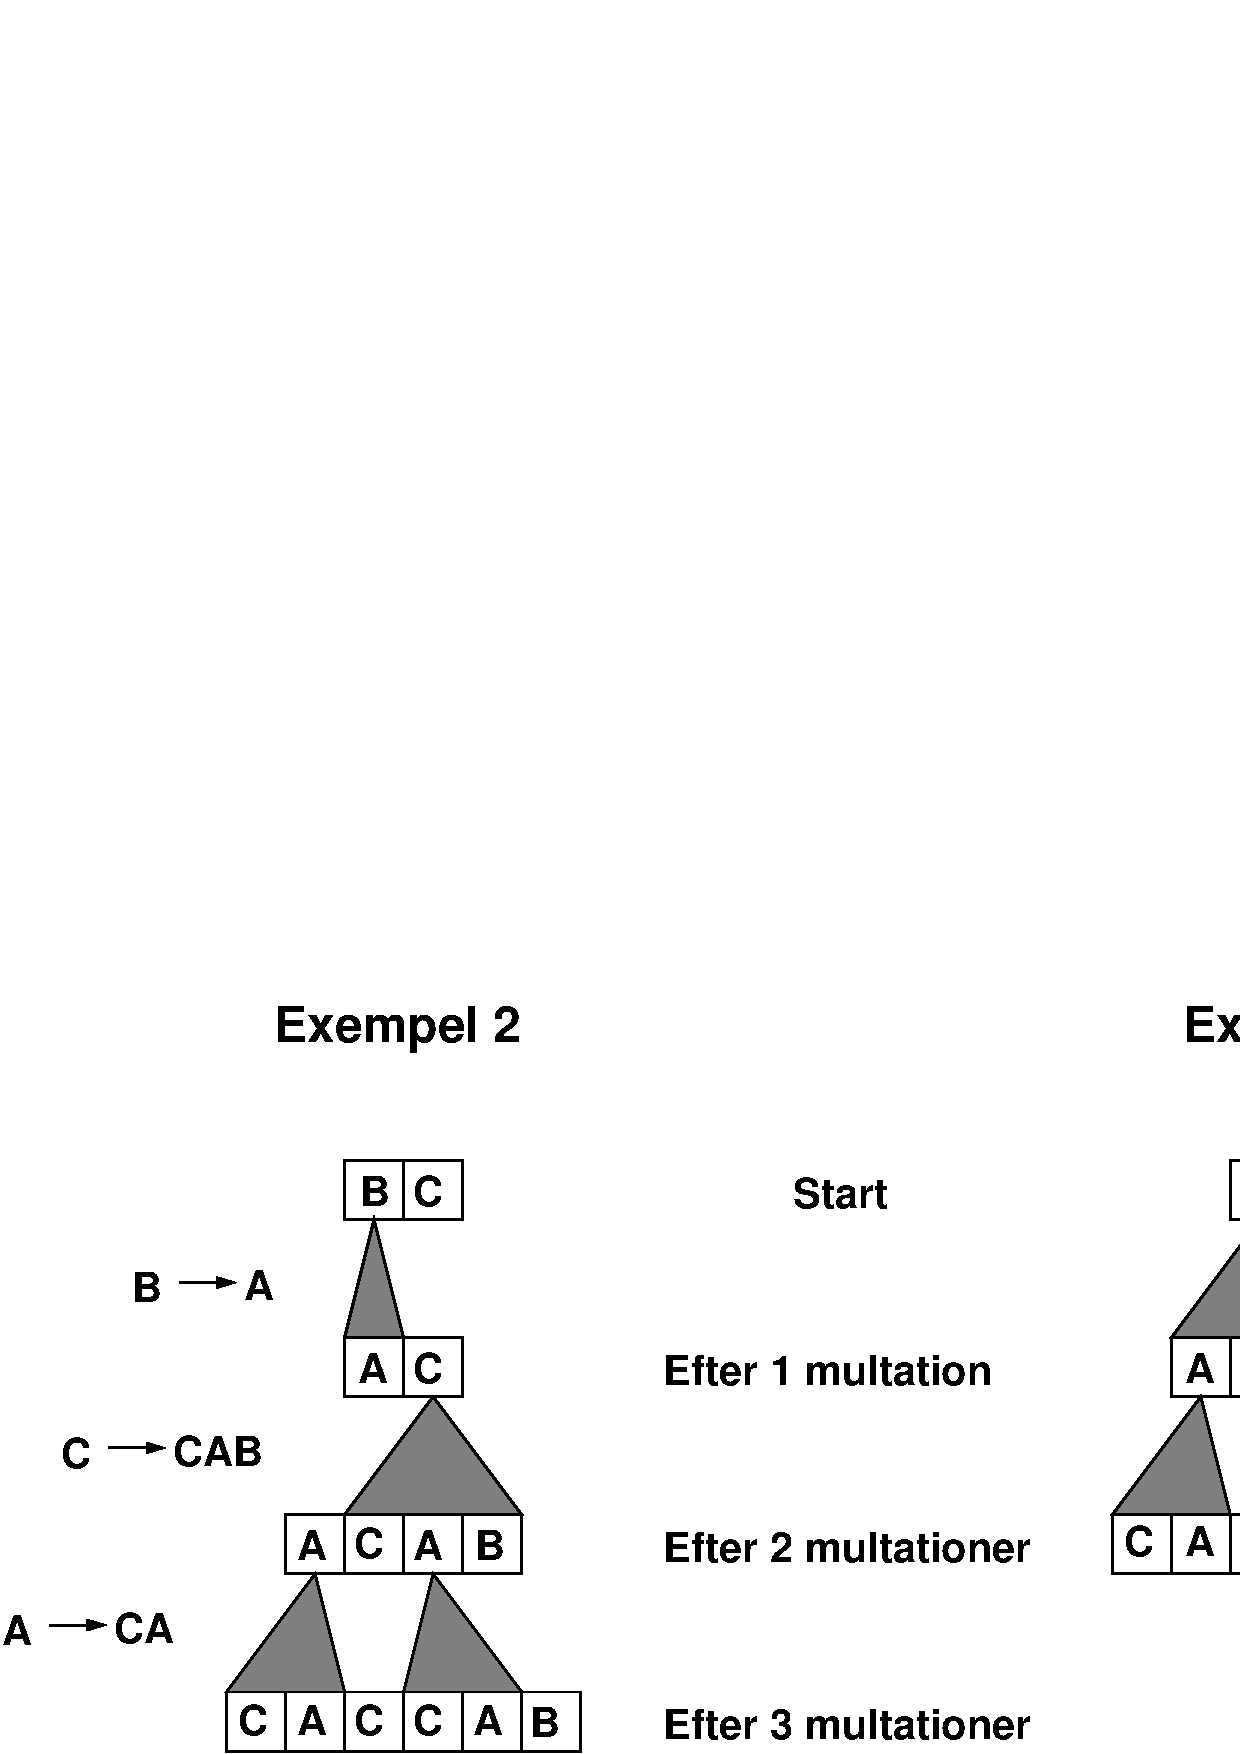
\includegraphics[width=0.9\textwidth]{multationer1.pdf}
\end{figure}
